% This is samplepaper.tex, a sample chapter demonstrating the
% LLNCS macro package for Springer Computer Science proceedings;
% Version 2.20 of 2017/10/04
%
\documentclass[runningheads]{llncs}
%
% Used for displaying a sample figure. If possible, figure files should
% be included in EPS format.
%
% If you use the hyperref package, please uncomment the following line
% to display URLs in blue roman font according to Springer's eBook style:
% \renewcommand\UrlFont{\color{blue}\rmfamily}
\usepackage[english]{babel}
\usepackage[utf8]{inputenc}
\usepackage{algorithm}
\usepackage{algpseudocode}
\usepackage{xspace}
\usepackage{mathtools}
\usepackage{amsmath}
\usepackage{graphicx}


\begin{document}
%
\title{Contribution Title\thanks{Supported by organization x.}}
%
%\titlerunning{Abbreviated paper title}
% If the paper title is too long for the running head, you can set
% an abbreviated paper title here
%
\author{First Author\inst{1}\orcidID{0000-1111-2222-3333} \and
Second Author\inst{2,3}\orcidID{1111-2222-3333-4444}}
%
\authorrunning{F. Author et al.}
% First names are abbreviated in the running head.
% If there are more than two authors, 'et al.' is used.
%
\institute{Princeton University, Princeton NJ 08544, USA \and
Springer Heidelberg, Tiergartenstr. 17, 69121 Heidelberg, Germany
\email{lncs@springer.com}\\
\url{http://www.springer.com/gp/computer-science/lncs} \and
ABC Institute, Rupert-Karls-University Heidelberg, Heidelberg, Germany\\
\email{\{abc,lncs\}@uni-heidelberg.de}}
%


\newcommand{\code}[1]{\text{#1}}
\newcommand{\inputF}{\ensuremath{F}}
\newcommand{\oneUIPClause}{\ensuremath{C_{1}}}
\newcommand{\iUIPClause}{\ensuremath{C_{i}}}
\newcommand{\assertionTrail}{\ensuremath{\phi}}
\newcommand{\LBD}{\text{LBD}}
\newcommand{\GAP}{\text{Gap}}
\newcommand{\IUIP}{\textbf{i-UIP}}
\newcommand{\IUIPPURE}{\textbf{Pure-i-UIP}}
\newcommand{\IUIPMIN}{\textbf{Min-i-UIP}}
\newcommand{\IUIPGreedy}{\textbf{i-UIP-Greedy}}
\newcommand{\IUIPActive}{\textbf{i-UIP-Inclusive}}
\newcommand{\IUIPDist}{\textbf{i-UIP-Exclusive}}
\newcommand\Set[2]{\{\,#1\mid#2\,\}}
\newcommand\Array[2]{[\,#1\mid#2\,]}
\newcommand\target{\textbf{Succ_t}}
\maketitle              % typeset the header of the contribution
%
\input{sections/abstract.tex}
\section{Introduction}

\input{sections/Preliminaries.tex}
\section{Find i-uip Clause} \label{sec:i-uip}
Classical CDCL SAT solvers analyze each conflict with 1-UIP resolution learning scheme to derive an asserting clause $\oneUIPClause$. Even though prior studies shows that further resolutions on $\oneUIPClause$ against the assertion trail $\assertionTrail$ cannot reduce the clause's literal block distance ($\LBD$), the resolutions could potentially reduce the clause's size. Clause size is an important quality measurement because a smaller clause 1) consumes less memory, 2) requires less steps to force a literal and 3) decreases the size of future conflict clauses.

Inspired by both $\LBD$ and clause size, i-UIP resolution learning attempts to resolve away literals in $\oneUIPClause$ against the assertion trail $\assertionTrail$ to minimize the clause size without increasing the clause's $\LBD$. The goal of i-UIP learning is to find a clause $\iUIPClause$ whose literals are either the unique implication points in their respective decision levels or are directly implied by literals from a foreign decision level. Alg. ~\ref{alg:i-uip} is a pseudo-code implementation of i-UIP learning. 


\begin{algorithm}[t]
\caption{\IUIP}\label{alg:i-uip}
\begin{algorithmic}[1]
\Require  $\oneUIPClause$ is a valid and minimized 1-UIP clause
\Require  $\assertionTrail$ is a valid assertion trail
\Procedure{\IUIP}{$\oneUIPClause, \assertionTrail$} 
    \State $\iUIPClause \gets \oneUIPClause $ \Comment{initialize i-UIP clause} \label{ln:init}
    \State \code{DecisionLvs} $\gets$ Decision levels in $\oneUIPClause$ in descending order
\For{$i \in \code{DecisionLvs}$} \label{ln:iterDecisionLvls}
    \State $L_{i} \gets \Set{l}{\code{level}(l) = i \wedge l \in \iUIPClause}$
    \While{$|\code{unmarked}(L_i)| > 1$} \label{ln:uip}
        \State $p \gets \text{lit with the highest trail position in } L_{i} $ \label{ln:trailaccess}
        \If{$\exists q \in \code{Reason}(\neg{p}, \assertionTrail) \cdot \code{level}(q) \not\in$ \code{DecisionLvs}} \label{ln:resolvable}
            \If{$\IUIPPURE$}
                \State Unresolve literals at level $i$  \label{ln:unresolve}
                \State Go to the next decision level $i$ \label{ln:abondon}
            \ElsIf{$\IUIPMIN$}
                \State $\code{Mark}(p)$ \label{ln:mark}
            \EndIf
        \Else 
            \State  $\iUIPClause \gets (\oneUIPClause ) \bowtie \code{Reason}(\neg{p}, \assertionTrail)$
           \State  $\code{Update}(L_{i})$
        \EndIf
    \EndWhile
\EndFor \label{ln:endCompleteResolution}
\\
\If{$\IUIPPURE$}\label{ln: 2ndMinStart}   \Comment{$\iUIPClause$ from $\IUIPPURE$ can be minimized}
    \State $\iUIPClause  \gets \textbf{Minimize}(\iUIPClause)$ 
\EndIf\label{ln: 2ndMinEnd}
\\
\If{$|\iUIPClause| < |\oneUIPClause|$} \label{ln:checkSize}
    \State \textbf{return} $\iUIPClause$
\Else
    \State \textbf{return} $\oneUIPClause$
\EndIf  \label{ln:cSizeCheck}
\EndProcedure
\end{algorithmic}
\end{algorithm}

The algorithm $\IUIP$ computes $\iUIPClause$ from (line~\ref{ln:init} to \ref{ln:endCompleteResolution}), and then returns the smaller clause between 
$\oneUIPClause$ and $\iUIPClause$ (line~\ref{ln:checkSize} to \ref{ln:cSizeCheck}). 
The algorithm first initializes $\iUIPClause$ with the minimized\cite{} $\oneUIPClause$. Next, the algorithm iterate through the decision levels of $\iUIPClause$ in descending order (line~\ref{ln:iterDecisionLvls}) and tries to find the unique implication point in each level (line~\ref{ln:uip}). Since $\IUIP$ needs to preserve $\iUIPClause$'s $\LBD$ during resolutions, before resolving away a target literal $p$, the algorithm preemptively checks whether the reasoning clause of $\neg{p}$ contains any literal $q$ from an unseen decision level (line~\ref{ln:resolvable}). If such a literal $q$ exists, then the algorithm cannot find the unique implication point (UIP) at the current level $i$ because resolving away $p$ will introduce $q$ into the clause and increases $\LBD$. One solution is to abandon level $i$ by reverting back to the state before any literal at level $i$ is resolved away (line~\ref{ln:unresolve}), and then move on to the next level (line~\ref{ln:abondon}). We denote $\IUIP$ learning with this solution as $\IUIPPURE$. The final $\iUIPClause$ produced by $\IUIPPURE$ will contains exactly one literal for levels where the LBD-persevering UIP exist. However, $\IUIPPURE$ does not minimize the number of literals in the decision levels where the LBD-preserving UIP does not exist, and clause minimization techniques\cite{} can be used to further reduce the clause size (line~\ref{ln: 2ndMinStart} to \ref{ln: 2ndMinEnd}). 

  When $\IUIP$ cannot resolve away a literal $p$ without increasing $\iUIPClause$'s LBD, instead of skipping the entire decision level $i$, a more practical solution $\IUIPMIN$ will mark and keep $p$ in $\iUIPClause$ (line~\ref{ln:mark}), and continue the resolutions at level $i$. $\IUIPMIN$ will ignore all the unsolvable literals and find the "local" unique implication point at every decision level.  The algorithm terminates when there is exactly one unmarked literal left for each decision level of $\iUIPClause$, representing the local unique implication points. The clause $\iUIPClause$ learnt by
  $\IUIPMIN$ is minimized\footnote{clause size cannot be reduced via minimization techniques\cite{}.}, we defer the minimization proof to Appendix~\ref{}.  

The core algorithm of $\IUIP$ as a clause reduction technique is simple. However, to make the algorithm a practical learning scheme that is compatible with modern SAT solvers, a number of issues need to be addressed. The rest of the section details the key optimizations and augmentations of $\IUIP$ as a practical clause learning scheme.

\subsection{Control i-UIP Learning}
This simple and greedy $\IUIP$ learning scheme can produce significantly smaller clause. However, when $\IUIP$ does not reduce the clause size, the cost of the additional resolution steps will hurt the solver's performance. Since resolution cannot reduce a clause's $\LBD$, The maximum size reduction from $\IUIP$ is the difference between the clause's size and $\LBD$, denote as the clause's gap value ($\GAP(\oneUIPClause) = |\oneUIPClause| - \LBD(\oneUIPClause)$). For an 1-UIP clause with a small $\GAP$, applying $\IUIP$ is unlikely to achieve cost effective results. Therefore, we propose a heuristic based approach to to enable and disable $\IUIP$ learning based on input clause's $\GAP$.

\begin{algorithm}[t]
\caption{Control-$\IUIP$}\label{alg:enableCondition}
\begin{algorithmic}[1]
\Require  $\oneUIPClause$ is a valid 1-UIP clause
\Require  $ t_{gap} \ge 0$ is a dynamically calculated gap threshold
\Procedure{Control-$\IUIP$}{$\oneUIPClause,  t_{gap}$} 
    \State $Gap \gets |\oneUIPClause| - \textit{LBD}(\oneUIPClause)$
     \If{$Gap > t_{gap}$} \label{ln:compareGap}
        \State $\iUIPClause \gets \IUIP(\oneUIPClause, \phi)$
        \State \textcolor{gray}{\textbf{I-UIP-Greedy}($\iUIPClause$ , $\oneUIPClause$)}  \Comment{additional clause selection policy, see sec~\ref{sec:greedy}}
        \If {$|\iUIPClause| < |\oneUIPClause|$} 
            \State $\text{Succeed} \gets \text{Succeed}+1$ \label{ln:updateS}
        \EndIf
        \State $\text{Attempted} \gets \text{Attempted}+1$ \label{ln:updateA}
     \EndIf
\EndProcedure
\end{algorithmic}
\end{algorithm}

Alg.~\ref{alg:enableCondition} compares the input $\oneUIPClause$'s $\GAP$ against a floating target threshold $t_{gap}$ (line~\ref{ln:compareGap}). The threshold $t_{gap}$ represent the expected minimal $\GAP$ required for $\oneUIPClause$ to achieve a predetermined success rate (80\%) from performing $\IUIP$ learning. 

The gap threshold $t_{gap}$ is initialized to 0, and is updated at every restart based on $\IUIP$'s success rate from the previous restart interval. More specifically, the algorithm collects the statistics of the number of $\IUIP$ learning attempted (line~\ref{ln:updateA} in alg.~\ref{alg:enableCondition}) and the number of attempts succeed (line~\ref{ln:updateS}) for each restart interval, and use them to calculate the success rate. If the success rate is below 80, the threshold $t_{gap}$ is increased to restrict $\IUIP$for the next restart interval. On the other hand, the threshold is decreased to encourage more aggressive $\IUIP$ learning for the next restart interval.

\[
    t_{gap}=
\begin{cases}
    t_{gap} + 1& \text{if } \frac{\text{Succeed}}{\text{Attempted}} < 0.8\\
    max(t_{gap} - 1, 0),              & \text{otherwise}
\end{cases}
\]

\subsection{Early stop i-UIP Learning}
At any point of $\IUIP$ learning, if the number of marked literals in $\iUIPClause$ (literals which are forced into the clause to preserve $\LBD$) exceeds the input clause $\oneUIPClause$'s $\GAP$, we can abort $\IUIP$ learning for $\oneUIPClause$ because the size of the final $\iUIPClause$ is at least the size of $\oneUIPClause$. The early stopping rule prevents solver from wasting time on traversing a large implication graph when $\IUIP$ has already failed.

\subsection{Greedy Active Clause Selection} \label{sec:greedy}
Even though $\IUIP$ learning can reduce the size of the learnt clause $\iUIPClause$, but it may introduce literals with low variable activity into $\iUIPClause$.  Inactive literals prevents the clause from being asserted to force literal implication. Therefore, a practical clause learning scheme should consider both size and variable activity. We propose an optional extension $\IUIPGreedy$ to filter out inactive $\oneUIPClause$.  

\begin{algorithm}[t]
\caption{$\IUIPGreedy$}\label{alg:greedySelection}
\begin{algorithmic}[1]
\Require  $\iUIPClause$ is a valid i-UIP clause
\Require  $\oneUIPClause$ is a valid 1-UIP clause
\Procedure{$\IUIPGreedy$}{$\iUIPClause, \oneUIPClause$} 
   \If{$|\iUIPClause| < |\oneUIPClause| \wedge (\code{AvgVarAct}(\iUIPClause) > \code{AvgVarAct}(\oneUIPClause)) $} \label{ln:checkSizeAndActivity}
    \State \textbf{return} $\iUIPClause$
\Else
    \State \textbf{return} $\oneUIPClause$
\EndIf  \label{ln:cSizeCheck}
\EndProcedure
\end{algorithmic}
\end{algorithm}

After computing the $\iUIPClause$, $\IUIPGreedy$ compares both the size and the average variable activity for $\oneUIPClause$ and $\iUIPClause$ (alg.~\ref{alg:greedySelection} at line~\ref{ln:checkSizeAndActivity}). The algorithm learns $\iUIPClause$ if the clause has smaller size and higher average variable activity. 

\subsection{Adjust Variable Activity} \label{sec: varajust}
Two popular branching heuristics for modern SAT solvers are VSIDS and LBR. Both heuristics increase 
the variable activity for all literals involved in resolutions during 1-UIP learning. Since $\IUIP$ extends 1-UIP with deeper resolutions against the trail, the variables activities for the fresh literals involved in the additional resolution steps need to be adjusted as well. We purpose two optional schemes for adjusting variable activities, $\IUIPActive$ and $\IUIPDist$. 

After learning $\oneUIPClause$ from 1-UIP scheme, $\IUIPActive$ collects all literals appear  in the the $\IUIP$ clause $\iUIPClause$, and increase their variable activity uniformly according to the current branching heuristic if the literals' variable activity have not yet been bumped during 1-UIP. The scheme does not bump variable activities for transient literals that are resolved away at non-conflicting level because, unlike transient literals at conflicting level, these literals cannot be re-asserted after the immediate backtracking. Notice that other post-analyze extensions such as Reason Side Rate (RSR) and Locality\cite{} can be applied after applying $\IUIPActive$ on $\iUIPClause$ so that no literal's variable activity is double bumped.

\[ \forall l \in  \iUIPClause \cdot NotBumped(var(l)) \implies  bumpActivity(var(l)) \]

$\IUIPDist$ collects literals appear exclusively in $\iUIPClause$ and bump their variable activity uniformly. It also find all the literals in $\oneUIPClause$ that are resolved away during $\IUIP$, and unbump their variable activity if they have been bumped during 1-UIP. The unbumped literals are no longer in the learned clause $\iUIPClause$, keep their variable activity bumped does not help solver to use $\iUIPClause$.

\[ \forall l_{i} \in  \iUIPClause \setminus \oneUIPClause \cdot bumpActivity(var(l_{i})) 
\]
\[ \forall l_{1} \in  \oneUIPClause \setminus \iUIPClause \cdot unbumpActivity(var(l_{1})) 
\]


\subsection{Integrate with Chronological Backtracking}
In SAT solver with chronological backtracking, literals on the assertion trail $\assertionTrail$ are not always sorted by decision levels. This change imposes a challenge to $\IUIP$ learning since the previous implementation relies on solver's ability to efficiently access all literals from any decision level in descending trail order (alg.~\ref{alg:i-uip} line~\ref{ln:trailaccess}). 

To mitigate this challenge, we modify the solver to track the precise trail position of all asserted literals with a single vector. We then build a priority queue $lit\_Order$ to manage literal's resolution order. The queue $lit\_Order$  prioritizes literals with higher decision level, and it favors literal with higher trail position when decision levels are tied. The order of $lit\_Order$  represents the correct resolution order of $\IUIP$ because 1) an asserted literal's decision level is the maximum level among all of its reasoning literals, and 2) an asserted literal always appears higher in the trail than its reasoning literal.  

\begin{algorithm}[t]
\caption{\IUIP-CB}\label{alg:i-uip-CB}
\begin{algorithmic}[1]
\Require  $\oneUIPClause$ is a valid 1-UIP clause
\Require  $\assertionTrail$ is a valid assertion trail
\Require  $lit\_Order$ is a priority queue
\Procedure{\IUIP-CB}{$\oneUIPClause, \assertionTrail, lit\_Order $} 
    \State ...
    \State $\iUIPClause \gets \oneUIPClause $ \Comment{initialize i-UIP clause}
    \State forall $l \in \oneUIPClause \cdot \code{Enqueu}(lit\_Order, l)$  \label{ln:enqueue}
    \State \code{DecisionLvs} $\gets \Set{\code{level}(l)}{l \in \oneUIPClause}$
    \While{$lit\_Order \neq \emptyset$} \label{ln:pop}
        \State $p \gets \code{dequeu}(lit\_Order, l) $ \label{ln:dequeue}
        \If{$\exists q \in \code{Reason}(\neg{p}, \assertionTrail) \cdot \code{level}(q) \not\in$ \code{DecisionLvs} \\ $\vee p$ is the last reminaing lit in its decision level } \label{ln:resolvable}
          \State Pass
        \Else 
            \State  $\iUIPClause \gets (\oneUIPClause ) \bowtie \code{Reason}(q, \assertionTrail)$
            \State   forall $l \in \code{Reason}(q, \assertionTrail) \cdot \code{Enqueu}(lit\_Order, l)$ \label{ln:reequeue}
        \EndIf
    \EndWhile
\State ...
\EndProcedure
\end{algorithmic}
\end{algorithm}

Alg.~\ref{alg:i-uip-CB} is the pesudo-code implementation of the augmented $\IUIP$ for chronological backtracking with the priority queue $lit\_Order$. The algorithm first populates $lit\_Order$ with all literals in $\oneUIPClause$ (line~\ref{ln:enqueue}), and then continuously pops literals until the queue is empty (line~\ref{ln:pop}). When a literal is resolved away, all of its reasoning literals are added into $lit\_Order$ if they are not already in the queue (line~\ref{ln:reequeue}). The algorithm will always terminate because a literal cannot entered the queue twice (guaranteed by the properties of the trail order) and there are finite amount of literals on the trail.
\section{Implementation and Experiments}

\subsection{Clause Reduction with $\IUIP$}
To evaluate $\IUIP$'s effectiveness as a clause reduction technique, we implement  $\IUIPPURE$ and $\IUIPMIN$ with Control-I-UIP and Early Stopping rules in Sec~\ref{sec:i-uip} on top of \text{\MapleBase} \cite{}, the winner of SAT Race 2015 application track.  We than compare the performance of the baseline $\MapleBase$ with $\MapleIUIPPURE$ and $\MapleIUIMIN$ on the full set of benchmarks from SAT RACE 2019 main track.

The benchmark contains 400 instances divided into two groups of 200, new and old, representing historical instances and fresh instances in the 2019 race, respectively. We randomly partition the old group instances into six partitions of size 30 and one partition of size 20. Each partition is then assigned to a XeonE5-2 CPU node with 16 cores (2 sockets 8 cores  and  1 thread) and 96649 MB memory. The new group is partitioned based on their contributor (e.g. Heule contributed 22 matrix multiplication instances), and each partition is assigned to a aforementioned CPU node. To speed up the experiment, we allow a CPU node to solver at most seven instances concurrently. 

Beside solved instances count and PAR-2 score, we additionally measure the average clause length and clause reduction ratio (both cumulative and non-cumulative)\footnote{The cumulative reduction ratio is obtained through learning all clauses with the target learning scheme; Therefore, the reduction is cumulative. The non-cumulative reduction ratio is obtained by running the target scheme for measurement only (the minimized 1-UIP clause is learned); Therefore, the reduction is not cumulative. }  for each instances. For $\MapleIUIPPURE$  and $\MapleIUIMIN$, we also captures the $\IUIP$ learning attempted rate and success rate.

\begin{figure} 
\begin{center}
\begin{tabular}{ | m{3.3cm} | m{2cm}| m{2cm} | m{2cm} | m{2.7cm} | } 
\hline
Solver & \# solved & PAR-2 & Clause Size & Cl Reduction\% \\ 
\hline
$\MapleBase$ & 221 (132, 89) & 5018.89 & 62.6 & 36.53\% \\ 
\hline
$\MapleIUIPPURE$ & \textbf{228} (135, 93) & \nf{4867.37} & 49.88 & 41.6\%  (42.72\%)\\ 
\hline
$\MapleIUIMIN$ & 226 (135, 91) & 4890.67 & \textbf{45.2} & \textbf{47.8\% (51.19\%)}\\ 
\hline
\end{tabular}
\end{center}
\caption{Benchmark results of $\MapleBase$ , $\MapleIUIPPURE$  and $\MapleIUIMIN$ on SAT2019 race main track.
CL Reduction\% is the clause size reduction ratio comparing to non-minimized 1-UIP clauses, and the values in the brackets are the non-cumulative reduction ratio.}
\label{fig:t1}
\end{figure}

Fig.~\ref{fig:t1} shows that $\IUIPPURE$ ($\IUIPPURE$) solved seven (five) more instances than the baseline solver with lower PAR-2 scores. $\IUIPPURE$ has marginally lower PAR-2 score than $\IUIPPURE$. Both $\IUIPPURE$ and $\IUIPMIN$ produce clause with significantly smaller size than 1-UIP by  20.4\% and 27.7\%, respectively. Fig.~\ref{fig:len_pdf} shows the probability density distribution (PDF) of the relative clause size of both i-uip learning schemes ($\IUIPPURE$ in red and $\IUIPMIN$ in green) for each instance. $\IUIPPURE$ ($\IUIPMIN$) produces shorter clauses for 77.7\% (88.5\%) of instances, and average relative reduction from 1-UIP is 16.7\% (18.6\%). Fig.~\ref{fig:len_compare} compares the absolute clause size of $\IUIPMIN$, $\IUIPPURE$ and 1-UIP, and it shows that both i-UIP learning schemes in general produce the smaller clauses, and the size reduction is more significant for instances with large average 1-UIP clause size. Moreover, $\IUIPMIN$ clauses (indicated in green) is consistently smaller than $\IUIPPURE$ clauses.

\begin{figure}
    \centering
    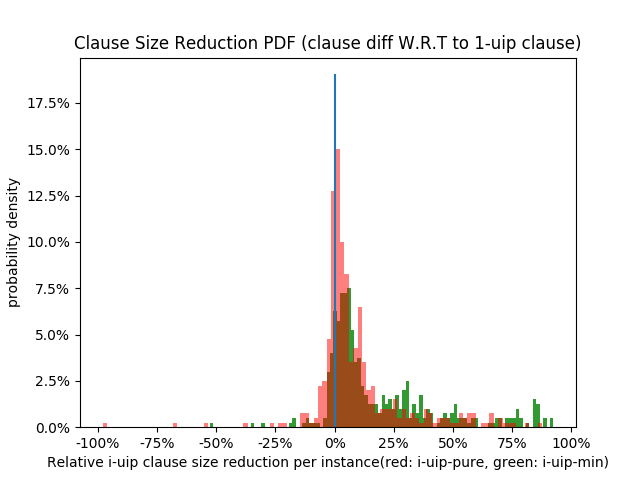
\includegraphics[width=0.8\textwidth,natwidth=610,natheight=642]{figures/clause_reduction_PDF.png}
    \caption{ Relative clause size reduction distribution. X axis indicates the relative size of difference between i-uip and 1-uip clauses (calculated as $\dfrac{|\oneUIPClause|-|\iUIPClause|}{|\oneUIPClause|}$ ) for each instance, and Y axis shows the probability density.}
     \label{fig:len_pdf}
\end{figure}
\begin{figure} \label{fig:len_compare}
    \centering
    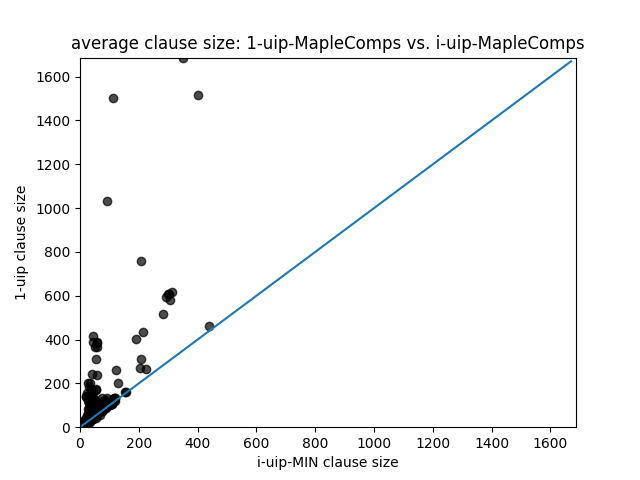
\includegraphics[width=0.8\textwidth,natwidth=610,natheight=642]{i-uip-sizes-compare.png}
    \caption{Average clause size comparison plot. Each point in the plot represents an instance. X and Y axis shows the clause length from $\IUIP$ and 1-UIP, respectively. Each green (red) dot represents an compared instance between $\MapleBase$ and $\MapleIUIMIN$ ($\IUIPPURE$). }
    \label{fig:len_compare}
\end{figure}
\nf{ Do we need this?
We additionally looked at the 14 instances solved by $\IUIPMIN$ but not by 1-UIP. $\IUIPMIN$ produces smaller clauses for all of them with average relative reduction of 22\% and maximum 77\% (30 vs 135). Seven out of 14 instances has size relative reduction over 30\%. For the 9 instances solved by 1-UIP but not by $\IUIPMIN$, $\IUIPMIN$ only produce smaller clause for three instances and with average relative reduction of 3.3\%.}

$\IUIPMIN$ outperformed $\IUIPPURE$ in clause size.  This results agrees with our observation in Fig.~\ref{fig:t2}: $\IUIPMIN$ attempted $\IUIP$ learning more frequently, and it is more likely to succeed.  

\begin{figure} 
\begin{center} 
\begin{tabular}{ | m{3.5cm} | m{5cm}| m{3.5cm} | } 
\hline
Solver & $\IUIP$ attempt rate & $\IUIP$ success rate  \\ 
\hline
$\MapleIUIPPURE$ & 16.1\% & 43.4\% \\ 
\hline
$\MapleIUIMIN$ & 28.8\% & 59.3\% \\ 
\hline
\end{tabular}
\end{center}
\caption{Compare $\IUIPPURE$ and $\IUIPMIN$ i-uip attempt rate and success rate. $\IUIPMIN$ scheme attempted $\IUIP$ more frequently, and it is more likely to successfully produce smaller $\iUIPClause$ clause .}
\label{fig:t2}
\end{figure}

A solver produce smaller clauses can construct smaller proofs. For UNSAT instances, we measure their DRUP\cite{} proof checking time as well as the size of the optimized DRUP proof. We used DART-trim \cite{} with 5000 timeout to check and optimize DRUP proofs. 

Fig.~\ref{fig:t3} shows that the optimized proof construct by $\IUIPMIN$ and $\IUIPPURE$ are significantly smaller than 1-UIP proofs. The relative proof size reduction roughly correlates to the average clause size reduction. Fig.~\ref{fig:proof_compare} shows the absolute proof size comparison results. 

\begin{figure} 
\begin{center} 
\begin{tabular}{ | m{3.5cm} | m{5cm}| m{3.5cm} | } 
\hline
Solver & optimized proof size (MB) & relative reduction size  \\ 
\hline
$\MapleBase$ & 613.9 & 0  \\ 
\hline
$\MapleIUIPPURE$ & 487.2 & 6.90\% \\ 
\hline
$\MapleIUIMIN$ & 413.2 & 17.18\% \\ 
\hline
\end{tabular}
\end{center}
\caption{Optimized UNSAT proof comparison for 1-UIP $\IUIPPURE$ and $\IUIPMIN$. Optimized proof size measures the average absolute proof size in MB, and relative reduction size measures the average relative reduction for all UNSAT instances.}
\label{fig:t3}
\end{figure}

\begin{figure}
    \centering
    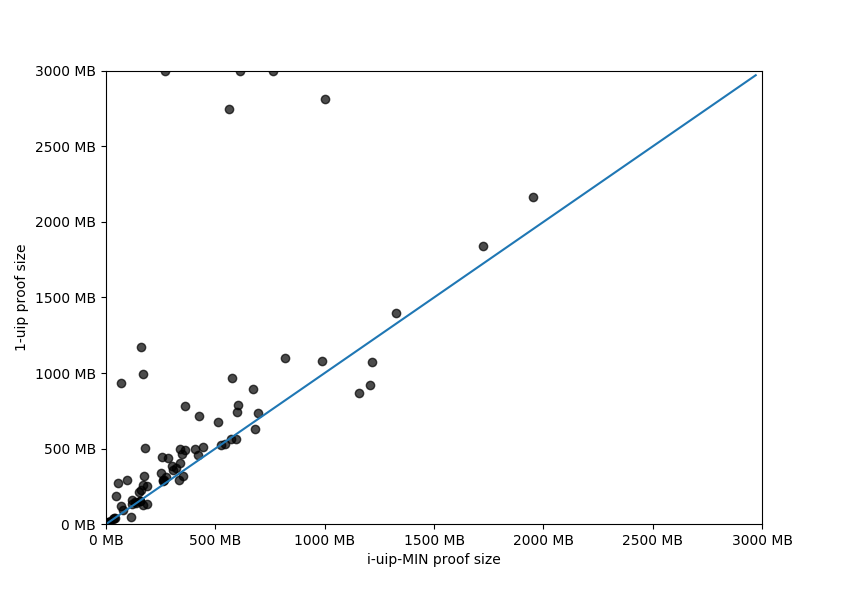
\includegraphics[width=0.8\textwidth,natwidth=610,natheight=642]{proof_size_compare.png}
    \caption{Average optimized proof size between 1-uip and $\IUIPMIN$.}
    \label{fig:proof_compare}
\end{figure}


\begin{figure} 
\begin{center}
\begin{tabular}{ | m{3.5cm} | m{4cm}| m{2cm} | m{2.75cm} |  } 
\hline
Solver & \# solved (SAT, UNSAT) & PAR-2 & Avg clause Size \\ 
\hline
1-UIP & 221 (132, 89)  & 5018.89 & 62.6  \\ 
\hline
\nf{$\IUIPPURE$} &\textbf{228} (135, \nf{93}) & 4867.37 & 49.88 \\
\hline
$\IUIPMIN$ & 226 (135, 91) & 4890.67 & 45.2 \\ 
\hline
$\IUIPGreedy$ & 226 (135, 91)  & \textbf{4866.94} & 47.7 \\
\hline
$\IUIPActive$ & 225 (\textbf{138}, 87) & 4958.49 & 52..12 \\
\hline
$\IUIPDist$ & 223 (134, 89) & 5015.23 & \textbf{43.2} \\
\hline
\end{tabular}
\end{center}
\caption{Benchmark results of $\MapleBase$ with 1-UIP, $\IUIPPURE$, $\IUIPMIN$, $\IUIPGreedy$,
$\IUIPActive$, and $\IUIPDist$ on SAT2019 race main track.}
\label{fig:t4}
\end{figure}

\subsection{$\IUIP$ as a Practical Learning Scheme}
To evaluate $\IUIP$'s effectiveness as a clause learning scheme, we re-implement $\IUIPMIN$ on $\MapleBase$ with the extensions mentioned in section~\ref{sec:i-uip}. We evaluated 1-UIP learning and five $\IUIP$ configurations ( $\IUIPMIN$, $\IUIPPURE$, $\IUIPGreedy$, $\IUIPActive$, and $\IUIPDist$) on the SAT Race 2019 main track benchmark and reported solved instances, PAR-2 score and average clause size. 

Fig.~\ref{fig:t4} summarizes the result of the experiment. Learning scheme $\IUIPPURE$ solved the most overall instances (228) and the most UNSAT instances (93). $\IUIPGreedy$ had the lowest PAR-2 score. $\IUIPActive$ solved the most SAT instances (138). $\IUIPDist$ produced the shortest average clause size, but solved the second least instances, one more instance than the baseline 1-UIP learning. All configurations of $\IUIP$ outperformed the baseline 1-UIP scheme in solved instances, PAR-2 score and average clause size.


\subsection{$\IUIP$ on Modern SAT solvers}
To validate $\IUIP$ as a generalizable learning scheme on modern SAT solvers, we re-implement $\IUIP$ on the winners of 2017, 2018 and 2019 SAT Race\cite{} and $\expSAT$\cite{} ($\expSATShort$). $\expSATShort$ is a top ten solver from 2019 SAT race which uses random walk simulation to help branching. We chose $\expSATShort$ because 1) it is a top solver in the 2019 SAT Race without using chronological backtracking; 2) the combination of random walk simulation and variable activity branching heuristic allows our learning schemes to partially sidestep the problem of variable activity. For each solver, we compare the base 1-UIP learning scheme against $\IUIPPURE$, $\IUIPMIN$ and the top two $\IUIP$ variants, $\IUIPGreedy$ and $\IUIPActive$, on the SAT Race 2019 main track benchmark. We report solved instances, PAR-2 score and the average clause size.

\begin{figure} 
\begin{center}
\begin{tabular}{ | m{3.7cm} | m{4cm}| m{2cm} | m{2.75cm} |  } 
\hline
Solver & \# solved (SAT, UNSAT) & PAR-2 & Avg clause Size \\ 
\hline
SAT 2017 Winner & & & \\
$\MapleSeven$ & 232 (135, 97) & 4755.96 & 61.9  \\ 
\hline
$\MapleSeven$-i-pure & \textbf{244 (146, 98)} +12 & \textbf{4504.18} & 43.76 \\
\hline
$\MapleSeven$-i-min & 240 (144, 96) +8 & 4601.25 & \textbf{36.97} \\ 
\hline
$\MapleSeven$-i-greedy & 237 (140, 97) +5 & 4678.434 & 43.62 \\ 
\hline
$\MapleSeven$-i-inclusive & 234 (137, 97) +2 & 4718.03 & 37.96 \\
\hline
\hline
SAT 2018 Winner & & & \\
$\MapleEightShort$ & 236 (138, 98) & 4671.81 & 61.69 \\
\hline
$\MapleEightShort$-i-pure & \textbf{241} (\textbf{142, 99}) +5 & \textbf{4598.18} & 44.19 \\
\hline
$\MapleEightShort$-i-min & 236 (141, 95) +0 & 4683.92 & 38.05 \\ 
\hline
$\MapleEightShort$-i-greedy & 240 (141, \textbf{99}) +4 & 4626.99 & 41.16 \\
\hline
$\MapleEightShort$-i-inclusive & 240 (\textbf{142}, 98) +4 & 4602.13 & \textbf{37.52} \\
\hline
\hline
SAT 2019 Winner & & & \\
$\MapleNineShort$ & 238 (140, \textbf{98}) & 4531.24 & 60.91 \\
\hline
$\MapleNineShort$-i-pure & 238 (140, \textbf{98}) +0 & 4519.08 &  43.32\\
\hline
$\MapleNineShort$-i-min & 244 (\textbf{148}, 96) +6 & \textbf{4419.84} & \textbf{36.88} \\
\hline
$\MapleNineShort$-i-greedy & 243 (146, 97) + 5 & 4476.73 & 40.65 \\
\hline
$\MapleNineShort$-i-inclusive & \textbf{243} (\textbf{148}, 95) +5 & 4455.76 & 37.02 \\
\hline
\hline
SAT 2019 Competitor & & &\\
$\expSATShort$ & 237 (137, 100)  & 4628.96 & 63.19 \\
\hline
$\expSATShort$-i-pure & 235 (136, 99) -2  & 4668.96 & 48.26 \\
\hline
$\expSATShort$-i-min & 241 (143, 98) +4 & 4524.28 & 46.29 \\ 
\hline
$\expSATShort$-i-greedy & 244 (143, \textbf{101}) +7 & \textbf{4460.92} & 47.25 \\
\hline
$\expSATShort$-i-inclusive & \textbf{245} (\textbf{146}, 99) +8 & 4475.76 & \textbf{45.33} \\
\hline
\end{tabular}
\end{center}
\caption{Benchmark results of 1-UIP, $\IUIPPURE$. $\IUIPMIN$, $\IUIPGreedy$ and $\IUIPActive$ on SAT2019 race main track.}
\label{fig:t5}
\end{figure}

Table~\ref{fig:t5} shows the benchmark result of $\IUIP$ configurations on different solvers. All four configurations of $\IUIP$ outperformed 1-UIP learning for the SAT 2017 race winner, $\MapleSeven$. More specifically, $\IUIPPURE$, $\IUIPMIN$, $\IUIPGreedy$ and $\IUIPActive$ solved 12, 8, 5 and 2 more instances, respectively, whiling producing smaller clauses. $\IUIPPURE$ solved more UNSAT and SAT instances while other configurations improved on solving SAT instances.  The improvement of $\IUIP$ is more significant on $\MapleSeven$ than on $\MapleBase$ for both solved instances and clause size reduction. This may suggests that $\IUIP$ and the recent learnt clause minimization approach~\cite{} synergies well because i-UIP clauses are shorter with more common literals which allows vivification~\cite{} to prune literals more aggressively through unit propagation. 

We observed significant improvement of $\IUIP$ for the SAT 2018 winner, $\MapleEightShort$. Three out of four $\IUIP$ configurations outperformed 1-UIP by 5, 4 an 4 instances, respectively. $\MapleEightShort$ improved from $\MapleSeven$ by using chronological backtracking (CB) for long distance backtracks. Therefore, we used $\IUIP$-CB extension for all $\IUIP$ configurations. The results indicates that the improvement of $\IUIP$ is slightly shadowed by the adoption of CB. More specifically, we believe CB prevents decision levels from being compressed through the process of backtracking and literal assertion. The shorter i-UIP clauses can bring related literals closer, which in turns compresses the assertion stack and the decision levels. However, since CB discourages long distance backtracking, the effect of learning shorter clauses is shadowed until a full restart.  We believe we have observed an interesting interaction effect that shows the limitations of both CB and $\IUIP$ learning for future research.  

$\IUIP$ learning schemes showed significant improvement for $\MapleNineShort$. Three out of four configurations improved solved instances by 6, 5 and 5 instances, respectively. $\MapleNineShort$ uses duplicate learning (DL) to prioritize clauses that are learned multiple times. $\IUIP$ and DL didn't synergies well possibly because i-UIP clauses are less likely to be duplicated. We observed that $\IUIPMIN$ ,in average, added 12\% less duplicated clauses into the core clause database than 1-UIP. One possible explanation is that $\IUIP$ learning can reduce an 1-UIP clause to different i-UIP clauses for different assertion trails. Therefore, the solver is less likely to learn the same i-UIP clauses.

We observed significant improvement of $\IUIP$ for $\expSATShort$, three out of four configurations of $\IUIP$ significantly outperformed 1-UIP learning by 4, 7 and 8 more instances, respectively, while producing smaller clauses. We expect all three configurations of $\IUIP$ to solve the similar amount of instances with close PAR-2 scores because the additional random walk exploration allows the learning schemes to partially sidestep the activity problem; hence, the learning adjustment for variable activities should have less impact on the solver's performance. However, we instead, observed that both $\IUIPGreedy$ and $\IUIPActive$ outperformed the default i-UIP learning scheme. One possible explanation is that $\IUIPGreedy$ and $\IUIPActive$ schemes could easily overcompensate variable activities for i-UIP clauses, and $\expSATShort$'s random walk exploration could use future search information to mitigate the negative effects of our overcompensation. 


%
\begin{thebibliography}{8}


\bibitem{ref_url1}
LNCS Homepage, \url{http://www.springer.com/lncs}. Last accessed 4
Oct 2017
\end{thebibliography}
\end{document}
